\documentclass[newpage]{homework}
\newcommand{\hwname}{Zooey Nguyen}
\newcommand{\hwemail}{zooeyn@ucla.edu}
\newcommand{\hwclass}{Astro 82}
\newcommand{\hwtype}{Homework}
\newcommand{\hwnum}{4}
\usepackage{siunitx}
\begin{document}
\maketitle


\question
Thermal timescale of Vega.
\begin{align*}
    t_t	&=	\frac{M/M_\odot}{(R/R_\odot)^2(L/L_\odot)^2} \vdot \SI{2e7}{yr}	\\
    t_t	&=	\frac{2^2}{3^2 \vdot  60^2} \vdot \SI{2e7}{yr}	\\
    t_t &=  \boxed{\SI{2.5e3}{yr}}    \\
\end{align*}
Nuclear timescale of Vega.
\begin{align*}
    t_n	&=	\frac{M/M_\odot}{L/L_\odot} \vdot \SI{1e10}{yr}	\\
    t_n    &=	\frac{2}{60} \vdot \SI{1e10}{yr}	\\
    t_n    &=	\boxed{\SI{3.3e8}{yr}}	\\
\end{align*}


\question
For hydrogen and helium fusion to be releasing the same amounts of energy we need the ratio of hydrogen to helium fusion reactions to make them equal each other. Let $N_H, N_{He}$ be the number of fusion reactions for hydrogen and helium respectively.
\begin{align*}
    N_H \vdot \SI{26.732}{\MeV}	&=	N_{He} \vdot \SI{7.275}{\MeV}	\\
    \frac{N_H}{N_{He}}    &=	\frac{7.275}{26.732}	\\
    \frac{N_H}{N_{He}}    &=	0.272	\\
\end{align*}
So the number of helium fusion interactions is occuring at approximately 4x the rate of hydrogen fusion. However, one helium fusion interaction requires 3 helium nuclei, while one hydrogen fusion interaction requires 4 hydrogen protons. So the mass put into a helium fusion is $3 \vdot 4m_p = 12m_p$ while the mass put into a hydrogen fusion is $4 \vdot m_p = 4m_p$. The mass required for a helium interaction is 3x that of hydrogen fusion. Thus helium fusion is occurring at about \fbox{4/3} the rate per unit mass that hydrogen fusion is occurring per unit mass.

We can find the size of this star by using the blackbody equation for luminosity.
\begin{align*}
    L/L_\odot	&=	\frac{4\pi \sigma R^2 T^4}{4\pi \sigma R_\odot^2 T_\odot^4}	\\
    L/L_\odot   &=  \left(\frac{R}{R_\odot}\right)^2 \left(\frac{T}{T_\odot}\right)^4   \\
    \frac{100}{(4600/5800)^4} &=  \left(\frac{R}{R_\odot}\right)^2  \\
    R   &=  \boxed{250 R_\odot}
\end{align*}


\question
In the diagram we see how Nb$^{93}$ can be synthesised by both the s-process and the r-process.
\begin{figure}[htbp]
    \centering
    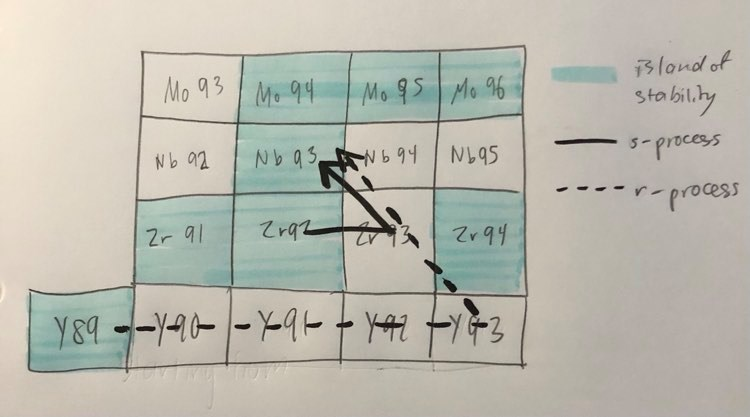
\includegraphics[width=0.8\textwidth]{nuclides.jpg}
\end{figure}

From the table provided in the problem set we can see an example of an element that cannot be produced by the s-process, Sr$^{84}$, as what has to be its progenitor, Rb$^{82}$, is unstable. We can also see that Mo$^{94}$ cannot be produced by the r-process, because decay along the r-process diagonal would run into Zr$^{94}$ first, and stabilise there.

\question
Use conservation of kinetic energy and add swept-up mass of the star to the surrounding medium of hydrogen before the snowplow phase.
\begin{align*}
    m_{tot}	&=	20 M_\odot + \frac{4}{3} (\SI{100}{\per\cubic\centi\metre}) m_p \pi (\SI{3}{pc})^3  	\\
    m_{tot} &=  \SI{5.915e32}{\kilogram} \\
\end{align*}
Assume that shell width is negligible and that negligible mass is swept up wrt total energy. Total energy of the shell is gravitational potential energy plus kinetic energy, which is conserved.
\begin{align*}
    U_{before} + K_{before}    &=	U_{after} + K_{after}	\\
    -\frac{GM^2}{2R_{before}} + \frac{Mv_{befor e}^2}{2}    &= -\frac{GM^2}{2R_{after}} + \frac{Mv_{after}^2}{2}	\\
    -\frac{G (\SI{5.915e32}{\kilogram})}{2 (\SI{3}{pc})} + \frac{(\SI{4e5}{\metre\per\second})^2}{2}    &= -\frac{G (\SI{5.915e32}{\kilogram})}{2R_{after}} + \frac{(\SI{1.5e3}{\metre\per\second})^2}{2}	\\
    R_{after}    &= \SI{2.46e11}{\metre}    \\
    R_{after}   &=  \boxed{\SI{8}{pc}}
\end{align*}

To get the mass swept up from when the radius was 3 pc to when the radius is 8 pc we add the mass of the swept-up shell.
\begin{align*}
    M	&=	\SI{5.915e32}{\kilogram} + \frac{4\pi}{3} (\SI{100}{\atomicmassunit\per\centi\metre^3}) ((\SI{8}{pc})^3 - (\SI{3}{pc})^3)	\\
    M   &=  \boxed{\SI{1.05e34}{\kilogram}}
\end{align*}
So it did turn out to be non-negligible mass. The actual $R_{after}$ is smaller than I calculated, then.
\end{document}
